%!TEX root = main.tex
\def\myscale{0.75}
\def\myscalematching{0.65}
\frametitle{Another example: From $11010$ to a perfect matching}
\newcommand\macrotile[1]{
     \def\south{}
     \def\east{}
     \def\north{}
     \def\west{} 
     \draw (\x + 0, \y) --  (\x+1,\y) node [pos=0.5,above] {\south} -- (\x+1,\y+1) node [pos=0.5,left] {\east} -- (\x+0,\y+1) node [pos=0.5,above] {\north} --  (\x + 0, \y)  node [pos=0.5,left] {\west};
}
%\newcommand\macropositivetileBinary{
%     \def\south{$0$}
%     \def\east{$0$}
%     \def\north{$1$}
%     \def\west{$1$} 
%     \draw (\x + 0, \y) --  (\x+1,\y) node [pos=0.5,above] {\south} -- (\x+1,\y+1) node [pos=0.5,left] {\east} -- (\x+0,\y+1) node [pos=0.5,above] {\north} --  (\x + 0, \y)  node [pos=0.5,left] {\west};
%}
\newcommand\macropositivetileBinaryWestEast{
     \def\south{}
     \def\east{\textcolor{blue}{\circled{$0$}}}
     \def\north{}
     \def\west{\textcolor{blue}{\circled{$1$}}}
     \draw (\x + 0, \y) --  (\x+1,\y) node [pos=0.5] {\south} -- (\x+1,\y+1) node [pos=0.5] {\east} -- (\x+0,\y+1) node [pos=0.5] {\north} --  (\x + 0, \y)  node [pos=0.5] {\west};
}
\newcommand\macropositivetileBinaryWest{
     \def\south{}
     \def\east{{$0$}}
     \def\north{}
     \def\west{\textcolor{blue}{\circled{$1$}}}
     \draw (\x + 0, \y) --  (\x+1,\y) node [pos=0.5] {\south} -- (\x+1,\y+1) node [pos=0.5] {\east} -- (\x+0,\y+1) node [pos=0.5] {\north} --  (\x + 0, \y)  node [pos=0.5] {\west};
}
\newcommand\macropositivetileBinaryEast{
     \def\south{}
     \def\east{\textcolor{blue}{\circled{$0$}}}
     \def\north{}
     \def\west{{$1$}} 
     \draw (\x + 0, \y) --  (\x+1,\y) node [pos=0.5] {\south} -- (\x+1,\y+1) node [pos=0.5] {\east} -- (\x+0,\y+1) node [pos=0.5] {\north} --  (\x + 0, \y)  node [pos=0.5] {\west};
}
\newcommand\macropositivetileBinaryWestNorth{
     \def\south{}
     \def\east{}
     \def\north{\textcolor{blue}{\circled{$1$}}}
     \def\west{\textcolor{blue}{\circled{$1$}}} 
     \draw (\x + 0, \y) --  (\x+1,\y) node [pos=0.5] {\south} -- (\x+1,\y+1) node [pos=0.5] {\east} -- (\x+0,\y+1) node [pos=0.5] {\north} --  (\x + 0, \y)  node [pos=0.5] {\west};
}
\newcommand\macropositivetileBinarySouthEast{
     \def\south{\textcolor{blue}{\circled{$0$}}}
     \def\east{\textcolor{blue}{\circled{$0$}}}
     \def\north{}
     \def\west{} 
     \draw (\x + 0, \y) --  (\x+1,\y) node [pos=0.5] {\south} -- (\x+1,\y+1) node [pos=0.5] {\east} -- (\x+0,\y+1) node [pos=0.5] {\north} --  (\x + 0, \y)  node [pos=0.5] {\west};
}
\newcommand\macropositivetileBinarySouth{
     \def\south{\textcolor{blue}{\circled{$0$}}}
     \def\east{}%{\textcolor{blue}{\circled{$0$}}}
     \def\north{}
     \def\west{} 
     \draw (\x + 0, \y) --  (\x+1,\y) node [pos=0.5] {\south} -- (\x+1,\y+1) node [pos=0.5] {\east} -- (\x+0,\y+1) node [pos=0.5] {\north} --  (\x + 0, \y)  node [pos=0.5] {\west};
}
\newcommand\macropositivetileBinarySouthNorth{
     \def\south{\textcolor{blue}{\circled{$0$}}}
     \def\east{}
     \def\north{\textcolor{blue}{\circled{$1$}}}
     \def\west{} 
     \draw (\x + 0, \y) --  (\x+1,\y) node [pos=0.5] {\south} -- (\x+1,\y+1) node [pos=0.5] {\east} -- (\x+0,\y+1) node [pos=0.5] {\north} --  (\x + 0, \y)  node [pos=0.5] {\west};
}

\newcommand\macronegativetileBinary{
     \def\south{$1$}
     \def\east{$1$}
     \def\north{$0$}
     \def\west{$0$} 
     \draw (\x + 0, \y) --  (\x+1,\y) node [pos=0.5] {\south} -- (\x+1,\y+1) node [pos=0.5] {\east} -- (\x+0,\y+1) node [pos=0.5] {\north} --  (\x + 0, \y)  node [pos=0.5] {\west};
}
\newcommand\macronegativetileBinaryWestEast{
     \def\south{}
     \def\east{\textcolor{blue}{\circled{$1$}}}
     \def\north{}
     \def\west{\textcolor{blue}{\circled{$0$}}}
     \draw (\x + 0, \y) --  (\x+1,\y) node [pos=0.5] {\south} -- (\x+1,\y+1) node [pos=0.5] {\east} -- (\x+0,\y+1) node [pos=0.5] {\north} --  (\x + 0, \y)  node [pos=0.5] {\west};
}
\newcommand\macronegativetileBinaryEast{
     \def\south{}
     \def\east{\textcolor{blue}{\circled{$1$}}}
     \def\north{}
     \def\west{{$0$}}
     \draw (\x + 0, \y) --  (\x+1,\y) node [pos=0.5] {\south} -- (\x+1,\y+1) node [pos=0.5] {\east} -- (\x+0,\y+1) node [pos=0.5] {\north} --  (\x + 0, \y)  node [pos=0.5] {\west};
}
\newcommand\macronegativetileBinaryWestNorth{
     \def\south{}
     \def\east{}
     \def\north{\textcolor{blue}{\circled{$0$}}}
     \def\west{\textcolor{blue}{\circled{$0$}}}
     \draw (\x + 0, \y) --  (\x+1,\y) node [pos=0.5] {\south} -- (\x+1,\y+1) node [pos=0.5] {\east} -- (\x+0,\y+1) node [pos=0.5] {\north} --  (\x + 0, \y)  node [pos=0.5] {\west};
}
\newcommand\macronegativetileBinarySouthEast{
     \def\south{\textcolor{blue}{\circled{$1$}}}
     \def\east{\textcolor{blue}{\circled{$1$}}}
     \def\north{}
     \def\west{} 
     \draw (\x + 0, \y) --  (\x+1,\y) node [pos=0.5,above] {\south} -- (\x+1,\y+1) node [pos=0.5,left] {\east} -- (\x+0,\y+1) node [pos=0.5,above] {\north} --  (\x + 0, \y)  node [pos=0.5,left] {\west};
}
\newcommand\macronegativetileBinarySouthEastNotcircled{
     \def\south{\textcolor{black}{{$1$}}}
     \def\east{\textcolor{black}{{$1$}}}
     \def\north{}
     \def\west{} 
     \draw (\x + 0, \y) --  (\x+1,\y) node [pos=0.5,above] {\south} -- (\x+1,\y+1) node [pos=0.5] {\east} -- (\x+0,\y+1) node [pos=0.5,above] {\north} --  (\x + 0, \y)  node [pos=0.5] {\west};
}

\newcommand\macronegativetileBinarySouthNorth{
     \def\south{\textcolor{blue}{\circled{$1$}}}
     \def\east{}
     \def\north{\textcolor{blue}{\circled{$0$}}}
     \def\west{} 
     \draw (\x + 0, \y) --  (\x+1,\y) node [pos=0.5] {\south} -- (\x+1,\y+1) node [pos=0.5] {\east} -- (\x+0,\y+1) node [pos=0.5] {\north} --  (\x + 0, \y)  node [pos=0.5] {\west};
}
\newcommand\macronegativetileBinaryNorthNotcircled{
     \def\south{\textcolor{black}{{$1$}}}
     \def\east{}
     \def\north{\textcolor{black}{{$0$}}}
     \def\west{} 
     \draw (\x + 0, \y) --  (\x+1,\y) node [pos=0.5] {\south} -- (\x+1,\y+1) node [pos=0.5] {\east} -- (\x+0,\y+1) node [pos=0.5] {\north} --  (\x + 0, \y)  node [pos=0.5] {\west};
}
\newcommand\macronegativetileBinaryWest{ % for a last tile
     \def\south{}
     \def\east{}
     \def\north{}
     \def\west{\textcolor{blue}{\circled{$0$}}}
     \draw (\x + 0, \y) --  (\x+1,\y) node [pos=0.5] {\south} -- (\x+1,\y+1) node [pos=0.5] {\east} -- (\x+0,\y+1) node [pos=0.5] {\north} --  (\x + 0, \y)  node [pos=0.5] {\west};
}
\newcommand\macronegativetileBinaryWestNotcircled{ % for a last tile
     \def\south{}
     \def\east{}
     \def\north{}
     \def\west{\textcolor{black}{{$0$}}}
     \draw (\x + 0, \y) --  (\x+1,\y) node [pos=0.5] {\south} -- (\x+1,\y+1) node [pos=0.5] {\east} -- (\x+0,\y+1) node [pos=0.5] {\north} --  (\x + 0, \y)  node [pos=0.5] {\west};
}

% begin snake graph 1011101100 or 2,3,1,2,3 (with 1 0 signs in interior)
 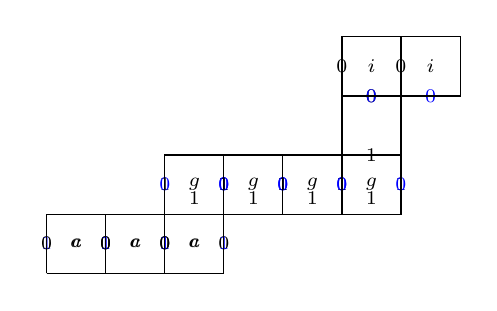
\begin{tikzpicture}[scale=\myscale,font=\scriptsize]
 \foreach \x in {0,1,...,2} % bottom row 
 {
\def\y{0}
     \ifthenelse{\x = 0}{\macropositivetileBinaryWest      \draw (\x + 0.5, \y+0.5) node {\boxed{$a$}};}{}
     \ifthenelse{\x = 1}{\macronegativetileBinaryEast}{}
     \ifthenelse{\x =2}{\macrotile{} %\macropositivetileBinaryWestNorth 
     \draw (\x + 0.5, \y+0.5) node {\boxed{$c$}};}{}
 }

\def\y{1}
 \foreach \x in {2,...,5} % second from bottom row
 {
     \ifthenelse{\x = 2}
     {\macronegativetileBinarySouthEastNotcircled }{}
     \ifthenelse{\x = 3}
     {\macropositivetileBinaryEast}{}
     \ifthenelse{\x = 4}
     {\macronegativetileBinaryWestEast}{}
     \ifthenelse{\x = 5}
     {\macrotile{} %\macropositivetileBinaryWestNorth 
     \draw (\x + 0.5, \y+0.5) node {\boxed{$g$}};
     }{}
 } 
 
\def\y{2}
 \foreach \x in {5} % third from bottom row
 {
     \macronegativetileBinaryNorthNotcircled{} %\macronegativetileBinarySouthNorth
 }  

\def\y{3}
\foreach \x in {5,6} % fourth from bottom row
{
     \ifthenelse{\x = 5}{\macropositivetileBinarySouth
     \draw (\x + 0.5, \y+0.5) node {\boxed{$i$}};}{}
     \ifthenelse{\x = 6}{\macronegativetileBinaryWestNotcircled }{}
 } 
 
\end{tikzpicture}

$\square_{\textcolor{blue}{1}} = \boxed{a}$, $\square_{\textcolor{blue}{1}} = \boxed{c}$ , $\square_{\textcolor{blue}{01}} = \boxed{g}$, and $\square_{\textcolor{blue}{0}} = \boxed{i}$.



\def\macrofilledtile{
\draw [fill=lightgray,opacity=0.99]  (\x + 0, \y) rectangle (\x+1,\y+1);
}
\def\macropositivetile{
     \def\south{}
     \def\east{}
     \def\north{}
     \def\west{} 
     \draw (\x + 0, \y) --  (\x+1,\y) node [pos=0.5,above] {\south} -- (\x+1,\y+1) node [pos=0.5,left] {\east} -- (\x+0,\y+1) node [pos=0.5,above] {\north} --  (\x + 0, \y)  node [pos=0.5,left] {\west};
}
\def\macronegativetile{
     \def\south{}
     \def\east{}
     \def\north{}
     \def\west{} 
     \draw (\x + 0, \y) --  (\x+1,\y) node [pos=0.5,above] {\south} -- (\x+1,\y+1) node [pos=0.5,left] {\east} -- (\x+0,\y+1) node [pos=0.5,above] {\north} --  (\x + 0, \y)  node [pos=0.5,left] {\west};
}
\def\matchingcolor{2pt}
% begin snake graph 1011101100 or 2,3,1,2,3 with matching generated by acgi
 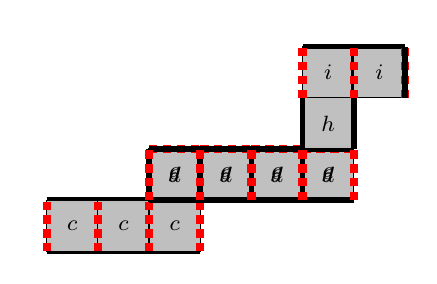
\begin{tikzpicture}[scale=\myscalematching,
 font=\footnotesize%\scriptsize
 ]
 \foreach \x in {0,1,...,2} % bottom row 
 {
%     \draw (\x + 0, 0) -- (\x+1,0) -- (\x+1,1)-- (\x+0,1) -- cycle;
\def\y{0}
     \ifthenelse{\x = 0 \OR \x =2}
     {
     \macropositivetile
     }{
     \macronegativetile
     }
     \ifthenelse{\x = 0 \OR \x =2}{\draw[line width=\matchingcolor] (\x + 0, \y+0) -- (\x+1,\y+0);}{} % south
     \ifthenelse{\x = 0}{\macrofilledtile \draw[line width=\matchingcolor] (\x + \y+0, \y+1) -- (\x+1,\y+1); }{} % north
     \ifthenelse{\x = 0}{\draw (\x + 0.5, \y+0.5) node {\boxed{$a$}}; }{}
     \ifthenelse{\x = 2}{ \macrofilledtile\draw (\x + 0.5, \y+0.5) node {\boxed{$c$}}; }{}
     
          \ifthenelse{\x = 0 \OR \x = 2}{\draw[red,densely dashed,line width=1.5*\matchingcolor] (\x+0, \y+0) -- (\x, \y+1);}{} % west
          \ifthenelse{\x = 0 \OR \x = 2}{\draw[red,densely dashed,line width=1.5*\matchingcolor] (\x+1, \y+0) -- (\x+1, \y+1);}{} % east
 }
\def\y{1}
 \foreach \x in {2,...,5} % second from bottom row
 {
     \ifthenelse{\x = 2 \OR \x = 3 \OR \x = 5}{\macrofilledtile}{}
     \ifthenelse{\x = 2}
     {\draw (\x + 0.5, \y+0.5) node {{$d$}}; }{}
     \ifthenelse{\x = 3}
     {\draw (\x + 0.5, \y+0.5) node {{$e$}}; }{}
     %\draw (\x + 0, \y) -- (\x+1,\y) -- (\x+1,\y+1)-- (\x+0,\y+1) -- cycle;
     \ifthenelse{\x = 3 \OR \x =5}
     {\macropositivetile}{\macronegativetile}
     \ifthenelse{\x = 2}{\draw[line width=\matchingcolor] (\x+0, \y+0) -- (\x, \y+1);}{} % west
%     \ifthenelse{\x = 2}{\draw[red, densely dashed, line width=1.5*\matchingcolor] (\x+0, \y+0) -- (\x+1, \y+0);}{} % south
     \ifthenelse{\x = 2}{\draw[red, densely dashed, line width=1.5*\matchingcolor] (\x+0, \y+1) -- (\x+1,\y+1);}{} % north
      \ifthenelse{\x = 3}{\draw[red, densely dashed, line width=1.5*\matchingcolor] (\x+1, \y) -- (\x+1,\y+1);}{} % east
      \ifthenelse{\x = 3}{\draw[line width=\matchingcolor] (\x+0, \y+0) -- (\x+1, \y+0);}{} % south
     \ifthenelse{\x = 3}{\draw[line width=\matchingcolor] (\x+0, \y+1) -- (\x+1,\y+1);}{} % north
      \ifthenelse{\x =5}{\draw[line width=\matchingcolor] (\x+0, \y+0) -- (\x+1, \y+0);}{} % south
      \ifthenelse{\x = 5}{\draw (\x + 0.5, \y+0.5) node {\boxed{$g$}}; }{}
      \ifthenelse{\x = 5}{\draw[red,densely dashed,line width=1.5*\matchingcolor] (\x+0, \y+0) -- (\x, \y+1);}{} % west
          \ifthenelse{\x = 5}{\draw[red,densely dashed,line width=1.5*\matchingcolor] (\x+1, \y+0) -- (\x+1, \y+1);}{} % east
 } 
\def\y{2}
 \foreach \x in {5} % third from bottom row
 {
     \macrofilledtile
     %\draw (\x + 0, \y) -- (\x+1,\y) -- (\x+1,\y+1)-- (\x+0,\y+1) -- cycle;
     \macronegativetile
     \ifthenelse{\x = 5}{\draw[line width=\matchingcolor] (\x+0, \y+0) -- (\x, \y+1);}{} % west
     \ifthenelse{\x = 5}{\draw[line width=\matchingcolor] (\x+1, \y) -- (\x+1,\y+1);}{} % east
%     \ifthenelse{\x = 5}{\draw[red,densely dashed,line width=1.5*\matchingcolor] (\x+0, \y+0) -- (\x+1, \y+0);}{} % south
     \draw (\x + 0.5, \y+0.5) node {{$h$}};
 }  
\def\y{3}
\foreach \x in {5,6} % fourth from bottom row
{
     %\draw (\x + 0, \y) -- (\x+1,\y) -- (\x+1,\y+1)-- (\x+0,\y+1) -- cycle;
     \ifthenelse{\x = 5}
     {\macropositivetile \macrofilledtile}{\macronegativetile}
     \ifthenelse{\x = 5}{\draw[line width=\matchingcolor] (\x+0, \y+1) -- (\x+1,\y+1);}{} % north
     \ifthenelse{\x = 5}{\draw[red,densely dashed,line width=1.5*\matchingcolor] (\x+0, \y+0) -- (\x, \y+1);}{} % west
          \ifthenelse{\x = 5}{\draw[red,densely dashed,line width=1.5*\matchingcolor] (\x+1, \y+0) -- (\x+1, \y+1);}{} % east

     \ifthenelse{\x = 6}{\draw[line width=\matchingcolor] (\x+1, \y) -- (\x+1,\y+1);}{} % east
%     \ifthenelse{\x = 6}{\draw[red,densely dashed,line width=1.5*\matchingcolor] (\x+0, \y+0) -- (\x+1, \y+0);}{} % south
%     \ifthenelse{\x = 6}{\draw[red,densely dashed,line width=1.5*\matchingcolor] (\x+0, \y+1) -- (\x+1,\y+1);}{} % north
     \ifthenelse{\x = 5}{\draw (\x + 0.5, \y+0.5) node {\boxed{$i$}}; }{}
 } 
\end{tikzpicture} % end of matching acgi
% begin snake graph 1011101100 or 2,3,1,2,3 with matching generated by acgi
 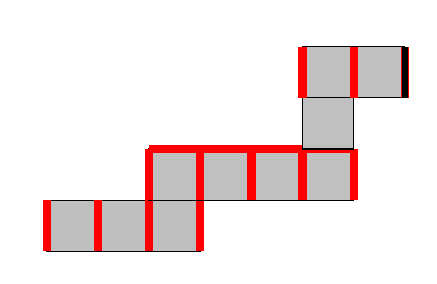
\begin{tikzpicture}[scale=\myscalematching,font=\scriptsize]
 \foreach \x in {0,1,...,2} % bottom row 
 {
%     \draw (\x + 0, 0) -- (\x+1,0) -- (\x+1,1)-- (\x+0,1) -- cycle;
\def\y{0}
     \ifthenelse{\x = 0 \OR \x =2}
     {
     \macropositivetile
     }{
     \macronegativetile
     }
%     \ifthenelse{\x = 0 \OR \x =2}{\draw[line width=\matchingcolor] (\x + 0, \y+0) -- (\x+1,\y+0);}{} % south
%     \ifthenelse{\x = 0}{ \draw[line width=\matchingcolor] (\x + \y+0, \y+1) -- (\x+1,\y+1); }{} % north
     \ifthenelse{\x = 0}{\macrofilledtile %\draw (\x + 0.5, \y+0.5) node {\boxed{$a$}};
      }{}
     \ifthenelse{\x = 2}{ \macrofilledtile %\draw (\x + 0.5, \y+0.5) node {\boxed{$c$}}; 
     }{}
     
          \ifthenelse{\x = 0 \OR \x = 2}{\draw[red,line width=1.5*\matchingcolor] (\x+0, \y+0) -- (\x, \y+1);}{} % west
          \ifthenelse{\x = 0 \OR \x = 2}{\draw[red,line width=1.5*\matchingcolor] (\x+1, \y+0) -- (\x+1, \y+1);}{} % east
 }
\def\y{1}
 \foreach \x in {2,...,5} % second from bottom row
 {
     \ifthenelse{\x = 2 \OR \x = 3 \OR \x = 5}{\macrofilledtile}{}
     %\ifthenelse{\x = 2}{\draw (\x + 0.5, \y+0.5) node {{$d$}}; }{}
     %\ifthenelse{\x = 3}{\draw (\x + 0.5, \y+0.5) node {{$e$}}; }{}
     %\draw (\x + 0, \y) -- (\x+1,\y) -- (\x+1,\y+1)-- (\x+0,\y+1) -- cycle;
     \ifthenelse{\x = 3 \OR \x =5}
     {\macropositivetile}{\macronegativetile}
%     \ifthenelse{\x = 2}{\draw[line width=\matchingcolor] (\x+0, \y+0) -- (\x, \y+1);}{} % west
%     \ifthenelse{\x = 2}{\draw[red, densely dashed, line width=1.5*\matchingcolor] (\x+0, \y+0) -- (\x+1, \y+0);}{} % south
     \ifthenelse{\x = 2}{\draw[red, line width=1.5*\matchingcolor] (\x+0, \y+1) -- (\x+1,\y+1);}{} % north
      \ifthenelse{\x = 3}{\draw[red, line width=1.5*\matchingcolor] (\x+1, \y) -- (\x+1,\y+1);}{} % east
%      \ifthenelse{\x = 3}{\draw[line width=\matchingcolor] (\x+0, \y+0) -- (\x+1, \y+0);}{} % south
%     \ifthenelse{\x = 3}{\draw[line width=\matchingcolor] (\x+0, \y+1) -- (\x+1,\y+1);}{} % north
%      \ifthenelse{\x =5}{\draw[line width=\matchingcolor] (\x+0, \y+0) -- (\x+1, \y+0);}{} % south
      %\ifthenelse{\x = 5}{\draw (\x + 0.5, \y+0.5) node {\boxed{$g$}}; }{}
      \ifthenelse{\x = 5}{\draw[red,line width=1.5*\matchingcolor] (\x+0, \y+0) -- (\x, \y+1);}{} % west
          \ifthenelse{\x = 5}{\draw[red,line width=1.5*\matchingcolor] (\x+1, \y+0) -- (\x+1, \y+1);}{} % east
 } 
\def\y{2}
 \foreach \x in {5} % third from bottom row
 {
     \macrofilledtile
     %\draw (\x + 0, \y) -- (\x+1,\y) -- (\x+1,\y+1)-- (\x+0,\y+1) -- cycle;
     \macronegativetile
%     \ifthenelse{\x = 5}{\draw[line width=\matchingcolor] (\x+0, \y+0) -- (\x, \y+1);}{} % west
%     \ifthenelse{\x = 5}{\draw[line width=\matchingcolor] (\x+1, \y) -- (\x+1,\y+1);}{} % east
%     \ifthenelse{\x = 5}{\draw[red,densely dashed,line width=1.5*\matchingcolor] (\x+0, \y+0) -- (\x+1, \y+0);}{} % south
    ;% \draw (\x + 0.5, \y+0.5) node {{$h$}};
 }  
\def\y{3}
\foreach \x in {5,6} % fourth from bottom row
{
     %\draw (\x + 0, \y) -- (\x+1,\y) -- (\x+1,\y+1)-- (\x+0,\y+1) -- cycle;
     \ifthenelse{\x = 5}
     {\macropositivetile \macrofilledtile}{\macronegativetile}
%     \ifthenelse{\x = 5}{\draw[line width=\matchingcolor] (\x+0, \y+1) -- (\x+1,\y+1);}{} % north
     \ifthenelse{\x = 5}{\draw[red,line width=1.5*\matchingcolor] (\x+0, \y+0) -- (\x, \y+1);}{} % west
          \ifthenelse{\x = 5}{\draw[red,line width=1.5*\matchingcolor] (\x+1, \y+0) -- (\x+1, \y+1);}{} % east

     \ifthenelse{\x = 6}{\draw[line width=\matchingcolor] (\x+1, \y) -- (\x+1,\y+1);}{} % east
%     \ifthenelse{\x = 6}{\draw[red,densely dashed,line width=1.5*\matchingcolor] (\x+0, \y+0) -- (\x+1, \y+0);}{} % south
%     \ifthenelse{\x = 6}{\draw[red,densely dashed,line width=1.5*\matchingcolor] (\x+0, \y+1) -- (\x+1,\y+1);}{} % north
     %\ifthenelse{\x = 5}{\draw (\x + 0.5, \y+0.5) node {\boxed{$i$}}; }{}
 } 
\end{tikzpicture} % end of matching acgi
